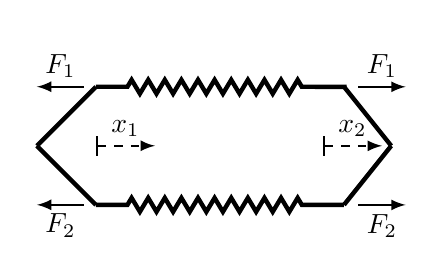
\begin{tikzpicture}[scale=1.5,xshift=0.5cm,every node/.style={outer sep=0pt,thick}]
	
	
	\tikzstyle{spring}=[ultra thick,decorate,decoration={zigzag,pre length=0.4cm,post length=0.5cm,segment length=6}]
	
	\tikzstyle{damper}=[ultra thick,decoration={markings,  
		mark connection node=dmp,
		mark=at position 0.5 with 
		{
			\node (dmp) [ultra thick,inner sep=0pt,transform shape,rotate=-90,minimum width=25pt,minimum height=8pt,draw=none] {};
			\draw [ultra thick] ($(dmp.north east)+(4pt,0)$) -- (dmp.south east) -- (dmp.south west) -- ($(dmp.north west)+(4pt,0)$);
			\draw [ultra thick] ($(dmp.north)+(0,-10pt)$) -- ($(dmp.north)+(0,10pt)$);
		}
	}, decorate]
	
	
	\
	\node (wall2) at (1.2cm,-4cm) [rotate=90, minimum width=1.5cm] {};
	
	\draw [spring] (-1cm,-4cm) -- (wall2.north) node[] {};
	\draw [latex-, thick] (-1.5cm,-4cm) --  ++(0.4cm,0cm) node[pos=.5,,above] {$F_1$};
	\draw [-latex, thick] (wall2.north) ++ (0.1,0cm) --  ++ (0.4cm,0cm) node[pos=.5,above] {$F_1$};
	
	\draw [|-latex, thick,dashed] (wall2.north) ++ (-0.2cm,-0.5cm) -- ++ (0.5cm, 0cm) node[above,midway] {$x_2$};
	
	\draw [|-latex, thick,dashed] (-1cm,-4.5cm) -- (-0.5cm,-4.5cm) node[above,midway] {$x_1$};
	
	\draw [spring] (-1cm,-4cm) ++ (0cm,-1cm) -- ++ (2.1cm,0cm) node[] {};
	\draw [-latex, thick] (wall2.north) ++ (0.1,-1cm) --  ++ (0.4cm,0cm) node[pos=.5,below] {$F_2$};
	\draw [latex-, thick] (-1.5cm,-5cm) --  ++(0.4cm,0cm) node[pos=.5,,below] {$F_2$};
		
	\draw [ultra thick] (-1cm,-4cm) -- (-1.5cm,-4.5cm) node[] {};
	\draw [ultra thick] (-1cm,-5cm) -- (-1.5cm,-4.5cm) node[] {};


\draw [ultra thick] (1.1cm,-4cm) -- (1.5cm,-4.5cm) node[] {};
\draw [ultra thick] (1.1cm,-5cm) -- (1.5cm,-4.5cm) node[] {};
\end{tikzpicture}